\chapter{Opis aplikacji}
\section{Ekran logowania}
\begin{figure}[htbp]
\centering
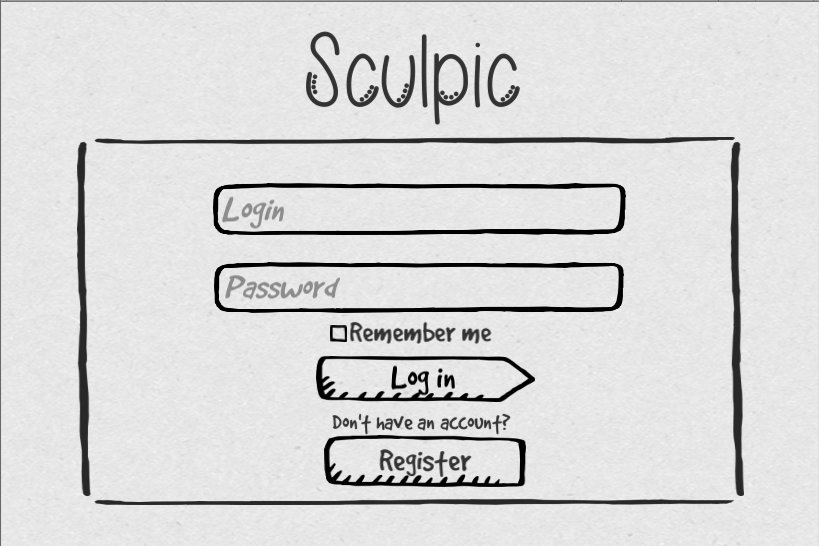
\includegraphics[width=\textwidth]{LogInScreen}
\caption{Ekran logowania.}
\label{fig:loginscreen}
\end{figure}

Ekran ten umożliwia zalogowanie się za pomocą danych do konta stworzonego wcześniej, bądź przejście do ekranu rejestracji. Pola tekstowe akceptują alfanumeryczne dane wejściowe, ponadto przy kliknięciu przycisku logowania następuje walidacja pól oraz wyświetlenie odpowiednich komunikatów w przypadku jej niepowodzenia. Możliwe jest także odznaczenie pola „Zapamiętaj mnie”, co sprawi, że przy ponownym uruchomieniu aplikacji nastąpi próba automatycznego logowania zapisanymi danymi. 

\begin{figure}[htbp]
\centering

\includegraphics[width=0.5\textwidth]{LoginValidation}
\caption{Walidacja pustego pola.}
\label{fig:loginvalidation}
\end{figure}

\section{Ekran rejestracji}
\begin{figure}[htbp]
\centering

\includegraphics[width=\textwidth]{RegisterScreen}
\caption{Ekran rejestracji.}
\label{fig:registerscreen}
\end{figure}

Ekran ten umożliwia założenie nowego konta poprzez podanie loginu oraz hasła. Kliknięcie przycisku „Zarejestruj” powoduje rejestrację, logowanie oraz przejście do ekranu wyboru pokoju. Reszta elementów zachowuje się tak jak na ekranie logowania, dochodzi jedynie dodatkowa walidacja – login musi składać się od 2 do 15 znaków, może zawierać jedynie litery oraz cyfry, hasła muszą do siebie pasować. W przypadku błędnie wprowadzanych danych wyświetlane są odpowiednie komunikaty.

\begin{figure}[htbp]
\centering

\includegraphics[width=0.5\textwidth]{SpecialCharsValidation}
\caption{Walidacja znaków specjalnych.}
\label{fig:specialcharsvalidation}
\end{figure}

\section{Ekran wyboru pokoju}
\begin{figure}[htbp]
\centering
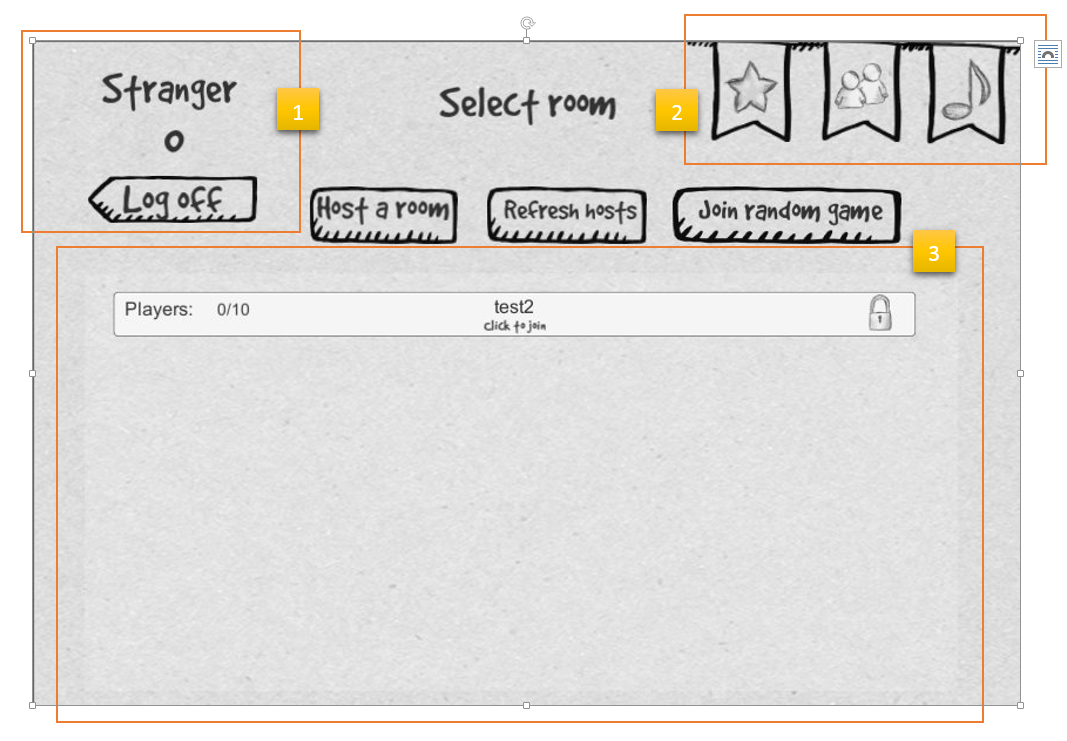
\includegraphics[width=\textwidth]{RoomChoiceScreen}
\caption{Ekran wyboru pokoju.}
\label{fig:roomchoicescreen}
\end{figure}

Jest to główny ekran aplikacji. Składa się on z trzech obszarów:
\begin{enumerate}
    \item Panel użytkownika – w nim wyświetlane są podstawowe informacje o użytkowniku, takie jak nazwa oraz ilość punktów rankingowych, zawiera on też przycisk umożliwiający wylogowanie (wyczyszczenie zapisanych danych dostępowych do konta oraz przejście do ekranu logowania). 
    \item Mini menu – zawiera przycisk przejścia do ekranu rankingu, przycisk prowadzący do ekranu zawierającego informacje o twórcach aplikacji oraz przycisk pozwalający włączyć lub wyłączyć dźwięki gry.
    \item Lista dostępnych pokojów – przyjmuje postać przewijanej listy złożonej z przycisków odpowiadającym pokojom, do których użytkownik może dołączyć. Kafelek pokoju zawiera podstawowe informacje takie jak liczba znajdujących się w nim graczy, limit graczy oraz nazwa. Ikonka kłódki znajdująca się po prawej stronie elementu informuje o tym, że dostęp do pokoju chroniony jest hasłem, w przeciwnym przypadku nie jest wyświetlana. Kliknięcie w przycisk powoduje połączenie się z pokojem oraz wejście do gry.
\end{enumerate}

Dodatkowo na ekranie znajduje się jeszcze przycisk pozwalający odświeżyć listę, przycisk umożliwiający przejście do ekranu tworzenia nowego pokoju oraz przycisk dołączenia do losowego pokoju niezabezpieczonego hasłem.

W przypadku próby wejścia do pokoju z ustawionym hasłem wyświetlane jest okno przedstawione na rysunku \ref{fig:roompassword}.

\begin{figure}[htbp]
\centering
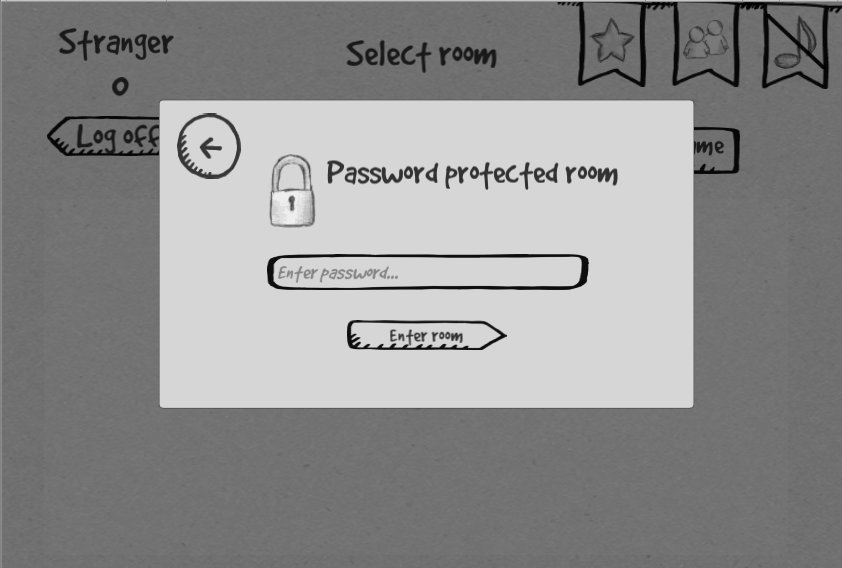
\includegraphics[width=\textwidth]{RoomPassword}
\caption{Okno umożliwiające wpisanie hasła.}
\label{fig:roompassword}
\end{figure}

\begin{figure}[htbp]
\centering

\includegraphics[width=0.5\textwidth]{RoomPasswordValidation}
\caption{Komunikat informujący o niepoprawnym haśle.}
\label{fig:roompasswordvalidation}
\end{figure}

\section{Ekran gracza zgadującego}
\begin{figure}[htbp]
\centering
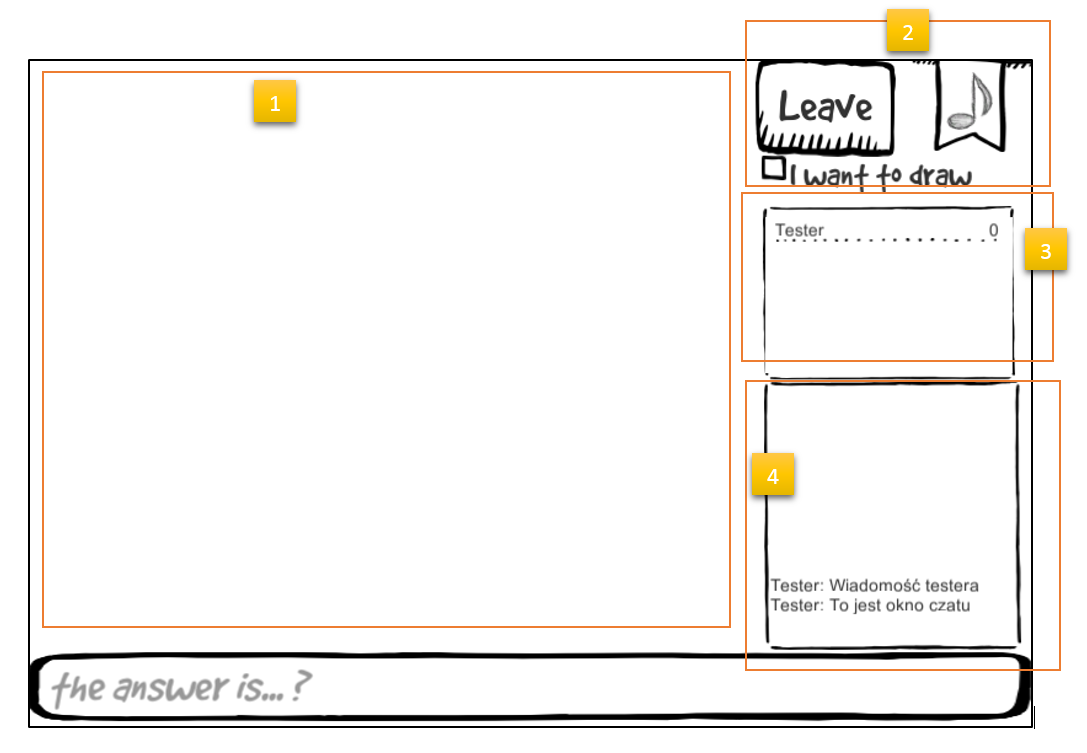
\includegraphics[width=\textwidth]{GuesserScreen}
\caption{Ekran gracza zgadującego.}
\label{fig:guesserscreen}
\end{figure}

Ten ekran widzą gracze, który aktualnie nie rysują. Złożony jest z następujących komponentów:
\begin{enumerate}
    \item Obszar gry – w tym miejscu jest wyświetlany obraz aktualnie stworzony przez rysującego. Każdy gracz może niezależnie obracać kamerą na swoim ekranie tak, by dało się przyjrzeć figurom z każdej strony. 
    \item Mini menu – zawiera przycisk umożliwiający opuszczenie gry, włączenie/wyłączenie dźwięku a także pole wyboru pozwalające na dołączenie bądź opuszczenie kolejki rysujących.
    \item Lista graczy – przewijana lista wyświetlająca nazwę oraz aktualną ilość punktów w grze każdego gracza w pokoju, posortowana malejąco według punktacji.
    \item Okno czatu – przewijana lista wiadomości, które użytkownicy wymieniają między sobą. Wyświetlane są tam też komunikaty systemu takie jak informacje o dołączających do pokoju graczach czy odgadniętym haśle. 
\end{enumerate}

Dodatkowo ekran zawiera pole umożliwiające pisanie wiadomości czatu, a tym samym odgadnięcie hasła.

\begin{figure}[htbp]
\centering
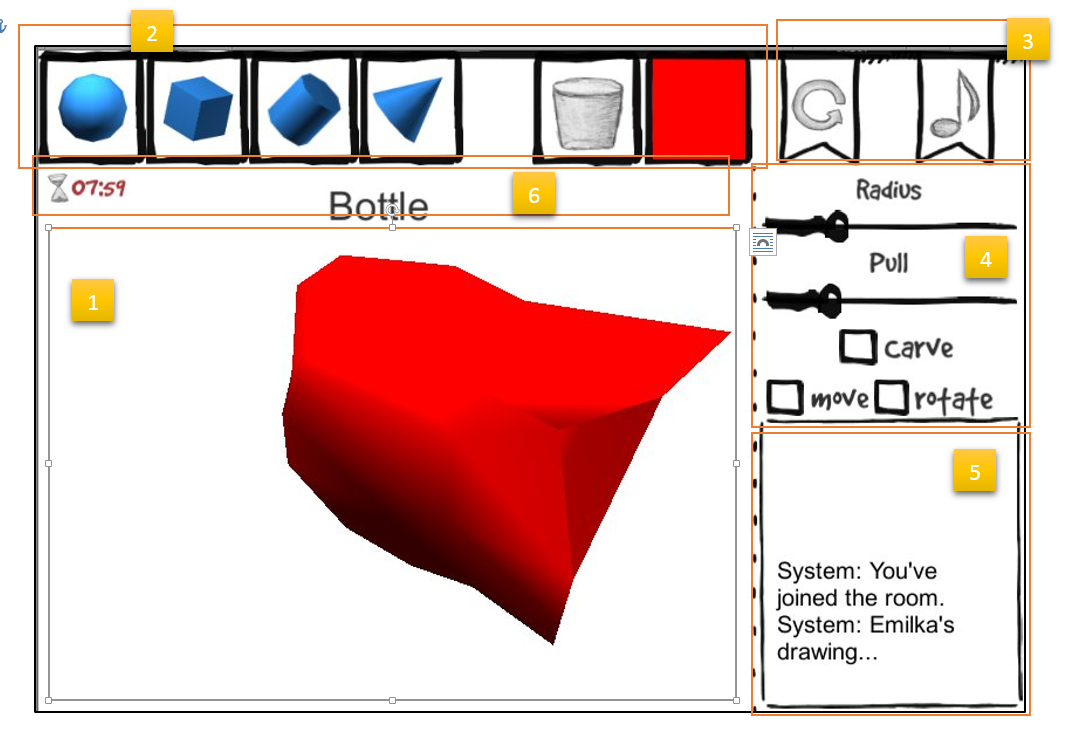
\includegraphics[width=\textwidth]{DrawerScreen}
\caption{Ekran gracza rysującego.}
\label{fig:drawerscreen}
\end{figure}

Ekran ten w danym momencie widzi tylko jedna osoba w pokoju – gracz aktualnie rysujący. Jest to najbardziej złożona scena aplikacji. Jej elementy są następujące:
\begin{enumerate}
    \item Pole modelowania – w tym obszarze pojawiają się nowo dodane figury, które można następnie modelować. Możliwe jest obracanie figur bądź poruszanie kamerą, umożliwiają to pola wyboru z obszaru numer 4.
    \item Przybornik – grupa przycisków po lewej stronie tego obszaru służy do wstawiania na scenę nowych figur. Dostępne są modele takie jak kula, sześcian, walec oraz stożek. Przyciski po prawej stronie umożliwiają wyczyszczenie sceny oraz zmianę koloru dodawanej figury.
    \item Mini menu – zawiera przycisk służący do odświeżenia sceny, czyli wysłania zmian do pozostałych graczy oraz przycisk włączenia/wyłączenia dźwięku.
    \item Ustawienia rysowania – suwaki umożliwiają zmianę parametrów skryptu sculptora – skryptu odpowiadającego za zmianę kształtu bryły. Możliwa jest zmiana zasięgu obszaru, na który wpływa sculptor oraz siły wybrzuszania. Pola wyboru pozwalają na tworzenie wgłębień a także zmianę pozycji oraz obracanie bryły.
    \item Okno czatu – statyczne okno czatu. Gracz rysujący nie ma możliwości pisania wiadomości, jednak może podglądać, czy gracze zgadujący są naprowadzani na poprawny trop odgadnięcia hasła.
    \item Panel informacyjny – w nim wyświetlany jest stoper odliczający czas pozostały na odgadnięcie hasła oraz samo hasło.
\end{enumerate}

\section{Ekran rankingu}
\begin{figure}[htbp]
\centering
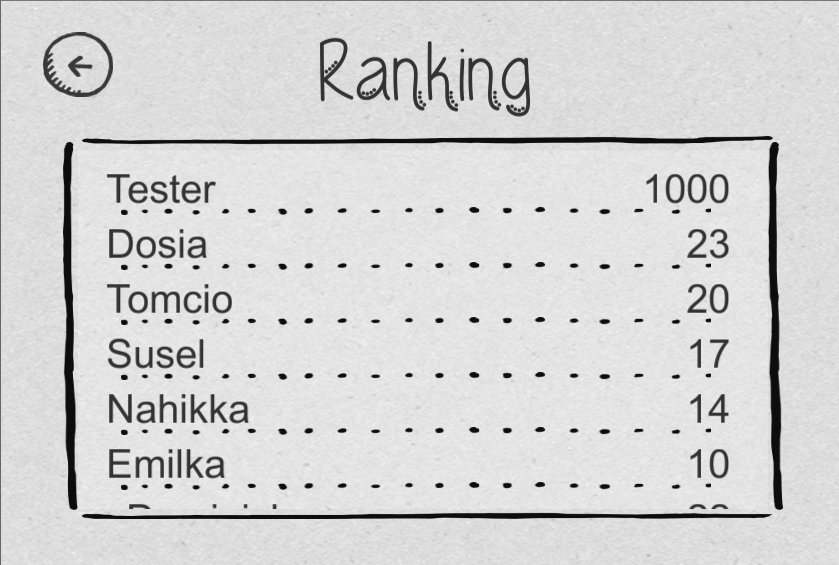
\includegraphics[width=\textwidth]{RankingScreen}
\caption{Ekran rankingu.}
\label{fig:rankingscreen}
\end{figure}

Ekran rankingu składa się z przesuwanej listy nazw graczy oraz wartości ich rankingów. Wyświetlane jest 20 najlepszych wyników w kolejności malejącej. Rekordy pobierane są z bazy za pomocą odpowiedniego serwisu.	